\documentclass[letterpaper, 12pt]{article}
\usepackage[margin=1in]{geometry}
\usepackage{amsmath}
\usepackage{amssymb}
\usepackage{xcolor}
\usepackage{graphicx}
\usepackage[center]{caption}
\usepackage{hyperref}
\usepackage{fancyhdr}
\usepackage{float}

\pagestyle{fancy}
\fancyhf{}
\rhead{
    Shengdong Li
    Table 7
    Calc 1
}
\rfoot{
    Page \thepage
}

\usepackage{indentfirst}
\setlength{\parindent}{2em}

\begin{document}
\title{Response to Katherine Peabody}
\author{by Shengdong Li}
\date{26 April 2020}
\maketitle

\section{Intro}
Hey Katherine! Good job on the initial post! It's great to see people embedding images, and the graph that you embedded helped me a lot with the visualization of the problem. The work was nice and clear as well. I looked through the entire discussion, but I couldn't find a single person with a problem that was different from mine to check using the disc/washer method that I didn't already do, so I decided to check your problem with a twist: flipping the two functions $y=\sqrt{x}$ and $y=x^2$ over the line $y=x$ and making it into a $dx$ problem.

\section{Solution}
To flip the two functions, I swapped $x$ with $y$ and solved for $y$.
\begin{align}
    y=\sqrt{x} & =x=\sqrt{y}         \\
               & =\boxed{y=x^{2}}    \\
    y=x^{2}    & =x=y^{2}            \\
               & =\boxed{y=\sqrt{x}}
\end{align}
I then graphed these two \textit{new} functions to better visualize the problem.
\begin{figure}[H]
    \begin{center}
        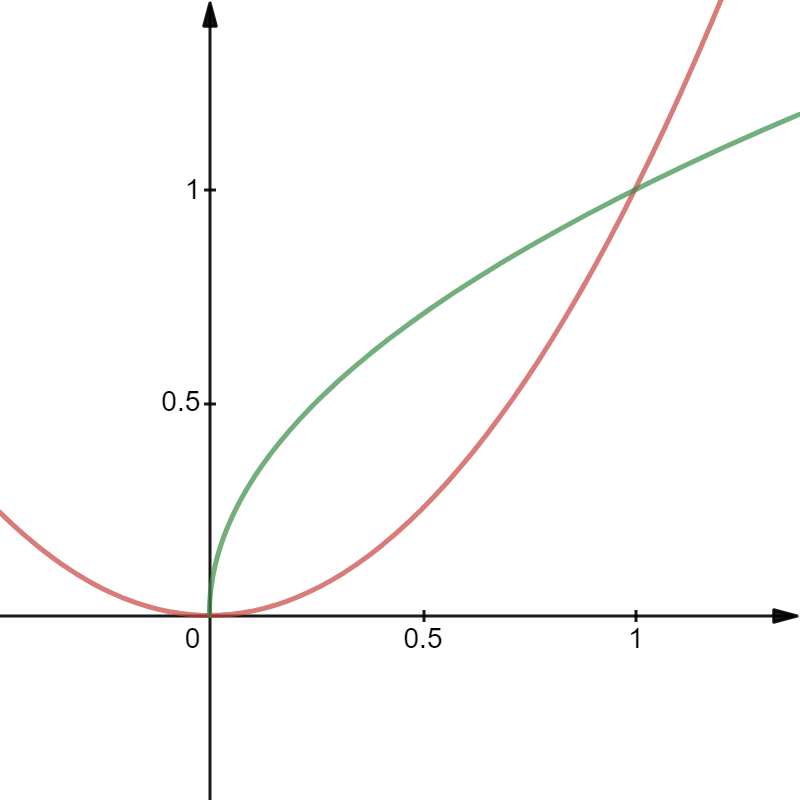
\includegraphics[scale=.3]{twoFunc.png}
        \caption{\textit{Red: $y=x^2$, Green: $y=\sqrt{x}$.} Desmos link \href{https://www.desmos.com/calculator/jbowfwj9rn}{\textcolor{blue}{here}}, or see embed below}
    \end{center}
\end{figure}
\begin{align}
    \intertext{From here, we'll just solve using the disc/washer method. First, since this is a $dx$ problem now, we don't have to put the equations in terms of $y$}
    \text{Outer Function: }                                               & y=\sqrt{x}                                                                                                                                        \\
    \text{Inner Function: }                                               & y=x^{2}
    \intertext{From the graph, it is clear that the left bound is $0$ and the right bound is $1$}
    a                                                                     & =0                                                                                                                                                \\
    b                                                                     & =1
    \intertext{Now we can just plugin to the disc/washer formula, making circular cross sections perpendicular to the $x$-axis.}
    \pi\int_{a}^{b}\left(f\left(x\right)^{2}-g\left(x\right)^{2}\right)dx & =\pi\int_{0}^{1}\left(\left(\sqrt{x}\right)^{2}-\left(x^{2}\right)^{2}\right)dx                                                                   \\
                                                                          & =\pi\int_{0}^{1}\left(x-x^{4}\right)dx                                                                                                            \\
                                                                          & =\pi\left(\frac{x^{2}}{2}-\frac{x^{5}}{5}\right)\Big|_{0}^{1}                                                                                     \\
                                                                          & =\pi\left(\frac{\left(1\right)^{2}}{2}-\frac{\left(1\right)^{5}}{5}-\left(\frac{\left(0\right)^{2}}{2}-\frac{\left(0\right)^{5}}{5}\right)\right) \\
                                                                          & =\pi\left(\frac{1}{2}-\frac{1}{5}\right)                                                                                                          \\
                                                                          & =\pi\left(\frac{5}{10}-\frac{2}{5}\right)                                                                                                         \\
                                                                          & =\frac{3\pi}{10}                                                                                                                                  \\
                                                                          & \approx\boxed{0.942}
\end{align}
\section{Conclusion}
It looks like we got the same answers! Good job on the initial post Katherine!
\end{document}